\documentclass{article} 
\usepackage[pdftex]{epsfig}
\usepackage{fancyhdr,subfig,graphicx,psfrag,amsfonts,textcomp,mathtools,amsmath,hyperref} 
\usepackage[margin=1.5cm]{geometry}

\title{Mandatory exercise 3 \\
Signal and Image Processing 2012} 
\author{Jens P. Raaby \\
\url{frn617@diku.dk}}

\begin{document} 
\maketitle

\section*{Question 3.1 - Noisy Signals}
Generating a 100 element vector of samples according to a given noise type was relatively easy with Matlab, with the exception of the Salt and Pepper noise which took some time to understand correctly. 

The file noiseGen1D.m contains a function to generate such samples. The histograms of the samples generated are shown in figure \ref{fig:q1} in the appendix (final page). 

In general, fitting parameters to a distribution will be more accurate with more samples. Therefore some of the inaccuracy of any estimates can be explained by the relatively small sample size.

\subsection*{Gaussian}
The Gaussian noise is generated using either of the functions randn and normrnd in MATLAB. It is relatively easy to estimate the parameters of the noisy signal, since they are defined:
\[
\mu = mean(sample)
\]
\[
\sigma = \sqrt{variance(sample)}
\]
Using these equations, I estimated the parameters at $\mu = -0.0528$ and $\sigma = 0.4758$.

\subsection*{Gamma}
Gamma noise parameters are slightly more complex to retrieve, but are still based on the mean and variance (equations 5.2-6 and 5.2-7 in Gonzalez \& Woods). With simple algebraic manipulation the terms $a$ and $b$ can be determined from the variance and mean:
%\begin{equation}
%\begin{array}{rl}
\[
a =  \frac {\mu} {\sigma ^2}
\]
\[
b =  \frac { \mu ^2} {\sigma ^2}
\]
%\end{array}
%\end{equation}
I found in practice that this returned some incorrect results (by testing different parameter values and comparing the estimates with those provided by Matlab's built in fitdist function). However for the given parameters (1,1) the error was not so great. I calculated $a=1.0343$ and $b=1.0801$.

\subsection*{Uniform}
In a similar manner to Gamma noise above, I rearranged the equations from Gonzalez and Woods to give:
\begin{equation}
\begin{array}{rl}
b = & \mu + \frac 1 2 {\sqrt{12\sigma ^2}}\\\\
a = & 2 \mu - b
\end{array}
\end{equation}
The results were quite accurate on the test data, giving $a=0.0667$ and $b=2.0825$.


\subsection*{Salt and pepper}
There was a lot of confusion and time wasting about this part of the assignment. Google did not help! 
My understanding of salt and pepper noise after reading more carefully (in particular the lecture slides provided at \url{http://cronos.rutgers.edu/~lrr/dsp\%20design\%20course/lectures/Lecture_IP5_2009.pdf}) is as follows:
The noise contains pepper (with intensity $a$)  with probability $P_a$, and salt (intensity $b$) with probability $P_b$. All other samples take some other value (with probability $1-(P_a + P_b)$). The original probabilities 0.1 and 0.2 made sense - 10\% of the signal should be pepper noise, and 20\% should be salt noise. The updated assignment changed the probabilities so that they sum to 1 (this is unnecessary, and means that the entire signal is noise!). 

Estimating the parameters is relatively easy when visually inspecting the histogram (see figure \ref{fig1:sandp}): there are two peaks at value 0 and 2, where one peak is twice the height of the other.

Calculating the parameters from the samples using the histogram (binned to the same size as the vector of samples) gave the following estimates:
$a = 0.0100$, $b = 1.9900$, $p_a = 0.3800$,$p_b =  0.6200$. These are close to the input parameters.

\subsection*{Using estimation with real images}
If the noise parameters of real images could be estimated using methods such as those I used above, it may be easier to restore the image to a less noisy condition. For example, if the salt and pepper noise parameters are estimated it should be relatively straightforward to replace the offending pixels (those with intensities $a$ and $b$) with the mean of the pixel neighbourhoods.
In the other types of noise, the pattern is more complex and (being stochastic) quite difficult to eliminate completely from inaccurate estimates. I would expect that using an iterative algorithm might be able to help in this instance. Once a basic estimate of noise parameters is known, subtract a m x n copy of the noise from the image (where the image size is m x n). Inspect the noise of the resulting image, and change each parameter in turn while observing the effect. If there is an improvement (reduction), keep adjusting the parameter in the same way until no improvements are observed. This 'gradient descent' approach would not be particularly practical in many cases.
A better approach would be to isolate a part of the image with relatively little detail (so that it is harder to confuse desirable pixels with noise) and estimate the noise parameters for only that area. Then one could use the parameters to tweak a noise removal filter.
 According to Gonzalez and Woods, various spatial filters  (such as mean) are typically used to smooth away noise from images. The order-statistic filters should yield even better results (for example the median filter mentioned in GW section 5.3.2).


\section*{Question 3.2 - Filtering out Noise}

\subsection*{house.tif}
Inspecting the histogram reveals what appears to be 2 spikes, suggesting salt and pepper noise. I used the imhist function to inspect the histogram and identified the pepper having value 6, and the salt having value 180. I tried using the wiener2 function, but as the noise is not so even (and constant power as the documentation states) the result was still peppery.
According to Gonzalez and Woods section 5.3.1, the contra harmonic mean filter is well suited to removing salt and pepper noise. I implemented this filter using Matlab's built in imfilter function. Figure \ref{q2:house} shows the results.
\begin{figure}[h]
\subfloat[Original image]{\label{fig2:house}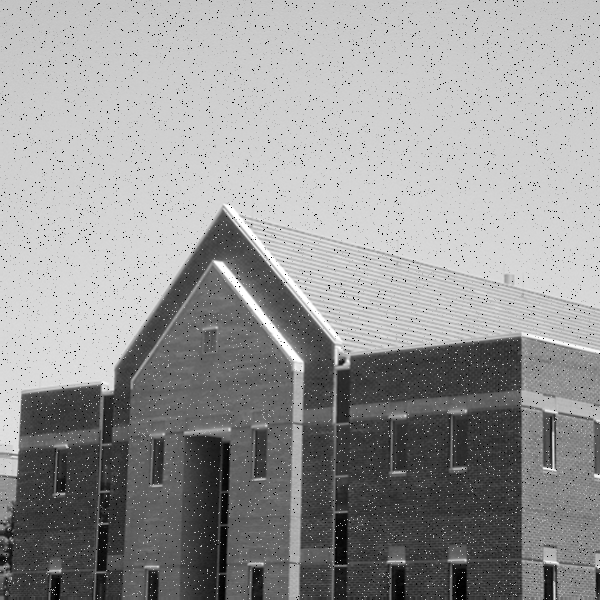
\includegraphics[width=0.3\textwidth]{q2-house.png}}\qquad
\subfloat[Pepper removed ($Q = 1.5$, $3x3$ mask)]{\label{fig2:housepep}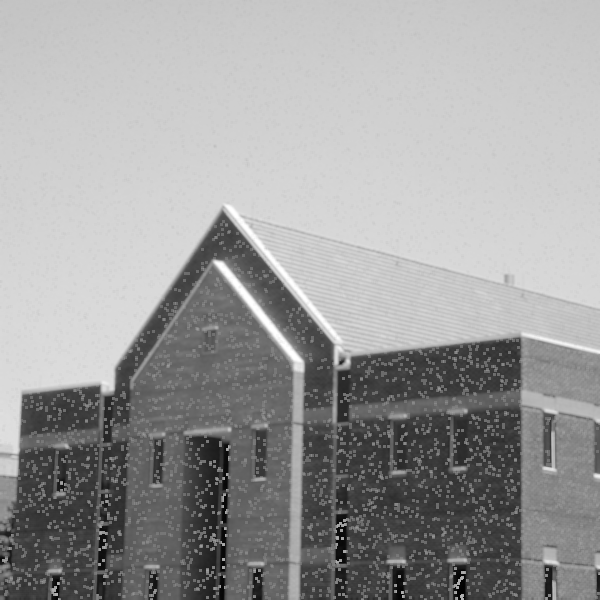
\includegraphics[width=0.3\textwidth]{q2-depeppered.png}}\qquad
\subfloat[Salt removed ($Q = -10$, $3x3$ mask)]{\label{fig2:housesalt}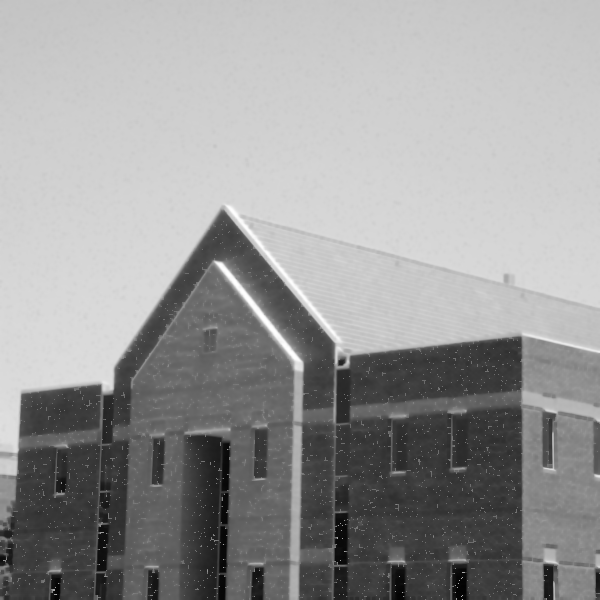
\includegraphics[width=0.3\textwidth]{q2-desalted.png}}
\caption{Applying the contra harmonic filter to house.tif}
\label{q2:house}
\end{figure}
The main problem with this filtering was that the two successive filterings reduced detail from the original image. The first filter ($Q=1.5$) increased blur in the darker areas (on the walls) thus spreading the salt noise. The second filter removed a lot of the salt but left some behind (thanks to the earlier blurring) and it also blurred the lighter areas. The final result is less sharp but cleaner at low magnification.

\subsection*{ic.tif}
This image has narrow dynamic range and a lot of fairly even looking noise. Inspecting the histogram in figure \ref{fig2:ichist} shows a shape that appears to have a Gaussian distribution.  Therefore the wiener2 function should be a better fit for this image. It looks at the neighbourhood for each pixel and adaptively removes noise. The result is shown (figure \ref{fig2:icwiener}) along with the histogram (figure \ref{fig2:icwhist}). There was not very much detail in the original image so the larger mask could be used to remove more noise.
\begin{figure}[h]
\subfloat[Original image]{\label{fig2:ic}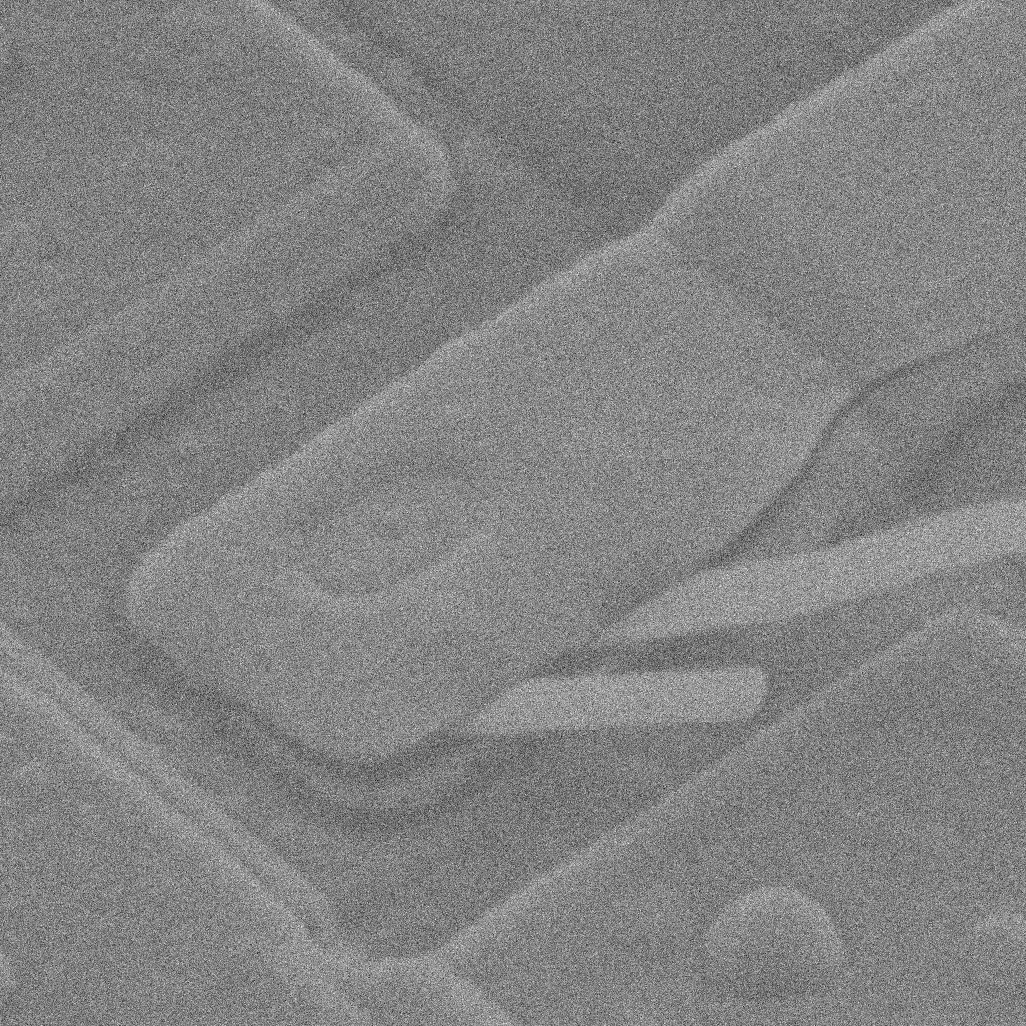
\includegraphics[width=0.22\textwidth]{q2-ic.png}}\qquad
\subfloat[Result of wiener2 function (15x15 mask)]{\label{fig2:icwiener}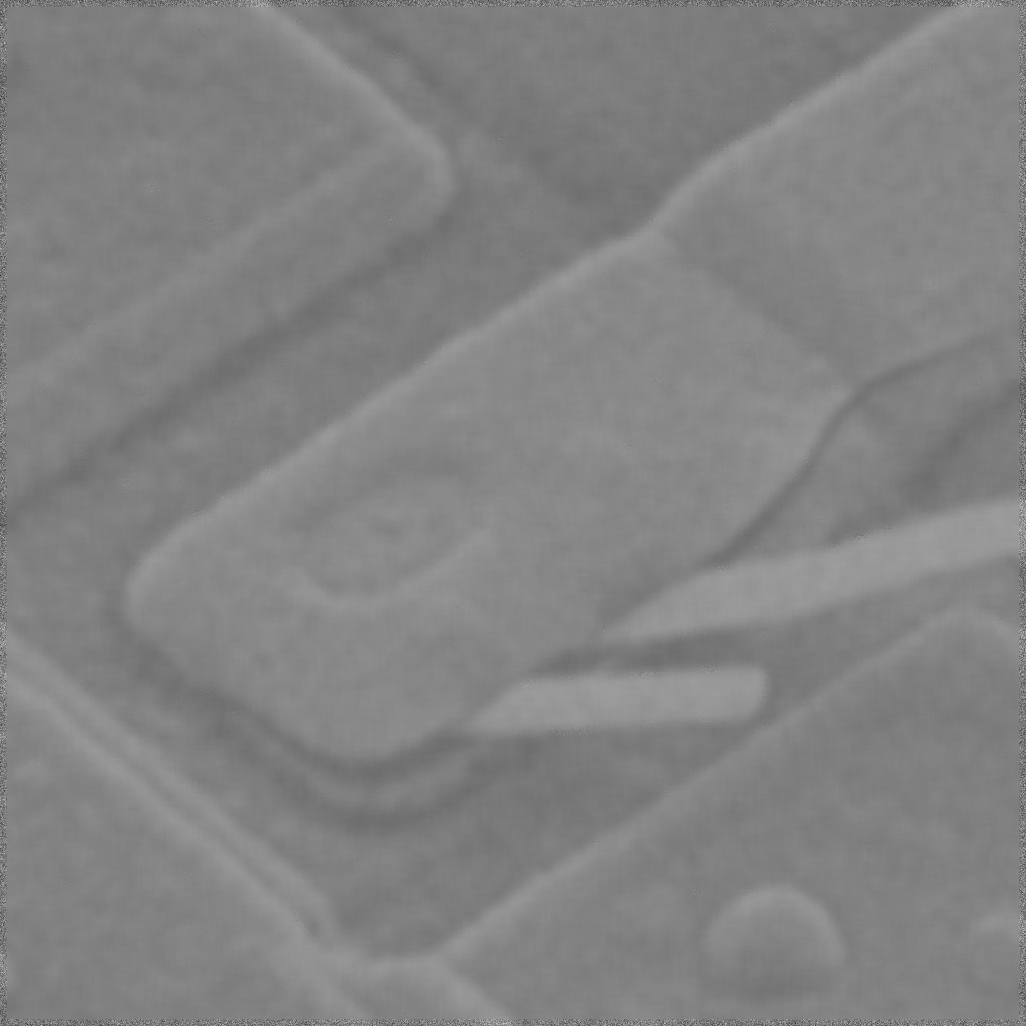
\includegraphics[width=0.22\textwidth]{q2-icwienered.png}}\qquad
\subfloat[Original histogram]{\label{fig2:ichist}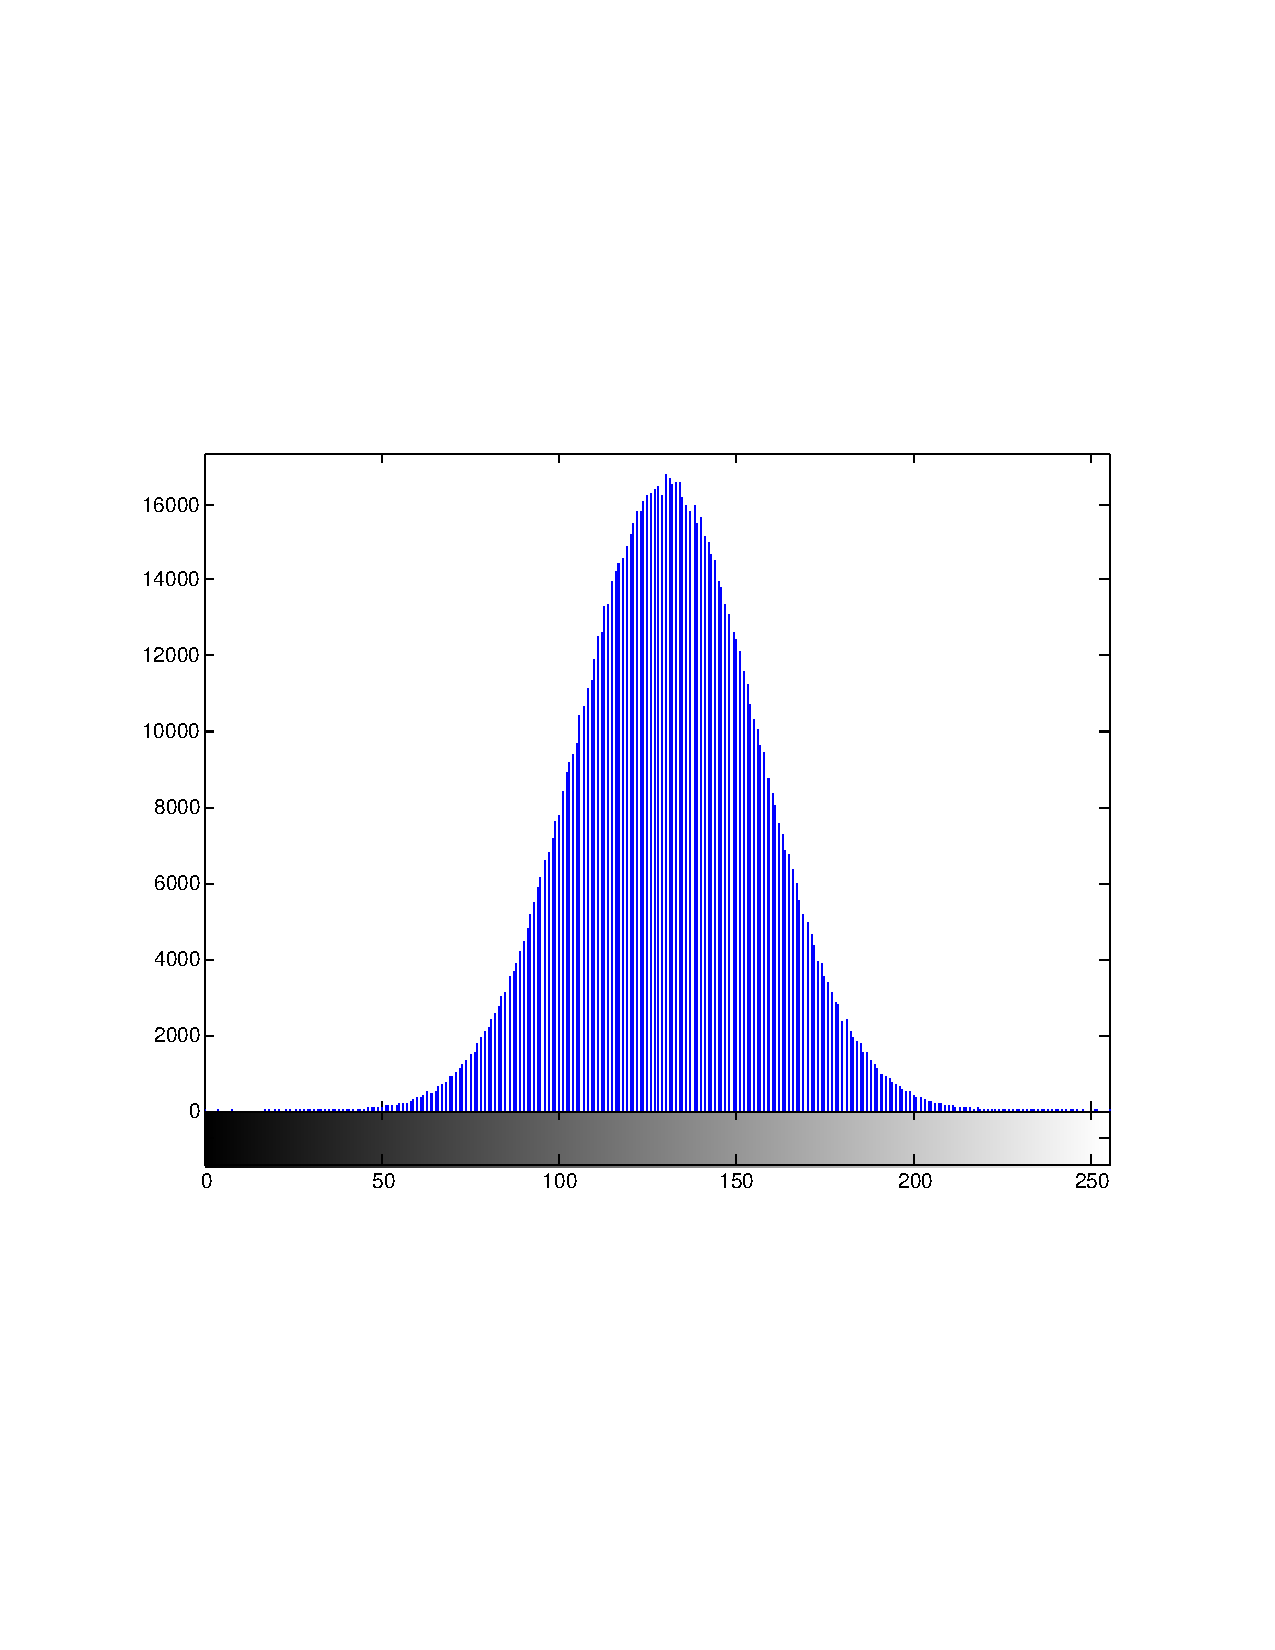
\includegraphics[width=0.22\textwidth]{q2-ichist.pdf}}
\subfloat[Histogram after filtering]{\label{fig2:icwhist}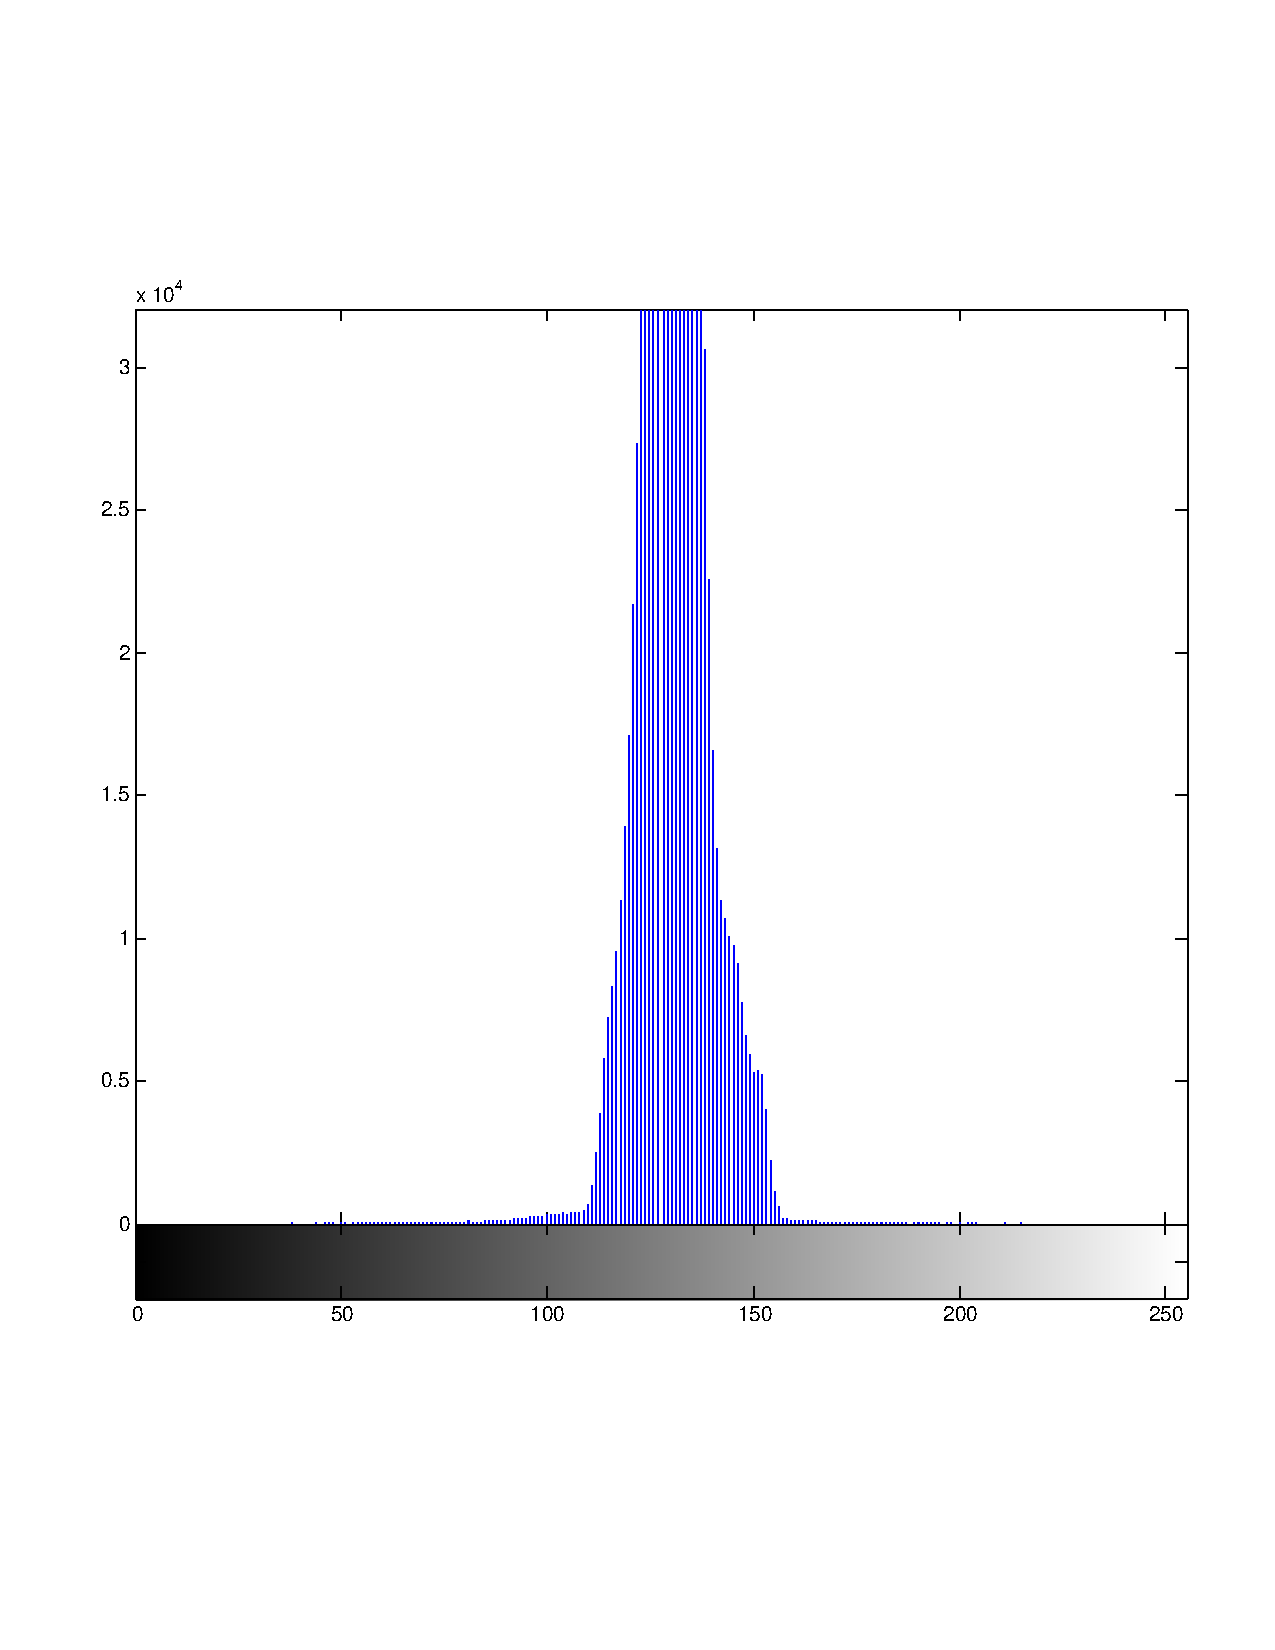
\includegraphics[width=0.22\textwidth]{q2-icwieneredhist.pdf}}
\caption{Applying the wiener2 function to ic.tif}
\label{q2:ic}
\end{figure}

\subsection*{boxes.tif}
This image's histogram suggests 2 kinds of noise: salt and pepper (in this case with only salt) and Gaussian. The salt noise is at the maximum frequency. I therefore decided to apply a combination of the contra harmonic filter for removing the salt noise and the wiener2 function for the Gaussian noise. I tried applying them in both orders, and found that removing the Gaussian noise first yielded better results. This is because the contra harmonic filter with negative power Q blurs the other noise in the lighter regions. The result (figure \ref{fig2:boxwienerch}) is not perfectly sharp but a vast improvement over the original.
\begin{figure}[h]
\subfloat[Original image]{\label{fig2:boxes}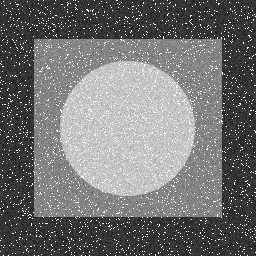
\includegraphics[width=0.3\textwidth]{q2-boxes.png}}\qquad
\subfloat[Result of wiener2 function (3x3 mask)]{\label{fig2:boxwiener}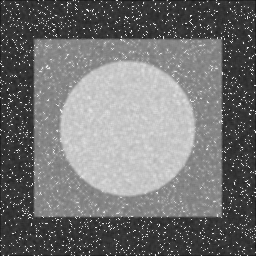
\includegraphics[width=0.3\textwidth]{q2-boxes-wienered.png}}\qquad
\subfloat[Result of contra harmonic function (3x3 mask, $Q=-10$) applied to figure \ref{fig2:boxwiener}]{\label{fig2:boxwienerch}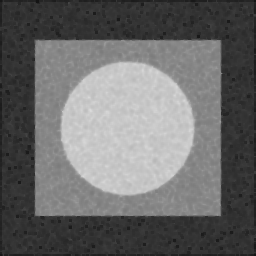
\includegraphics[width=0.3\textwidth]{q2-boxesdesalt.png}}\qquad
%\subfloat[Original histogram]{\label{fig2:boxhist}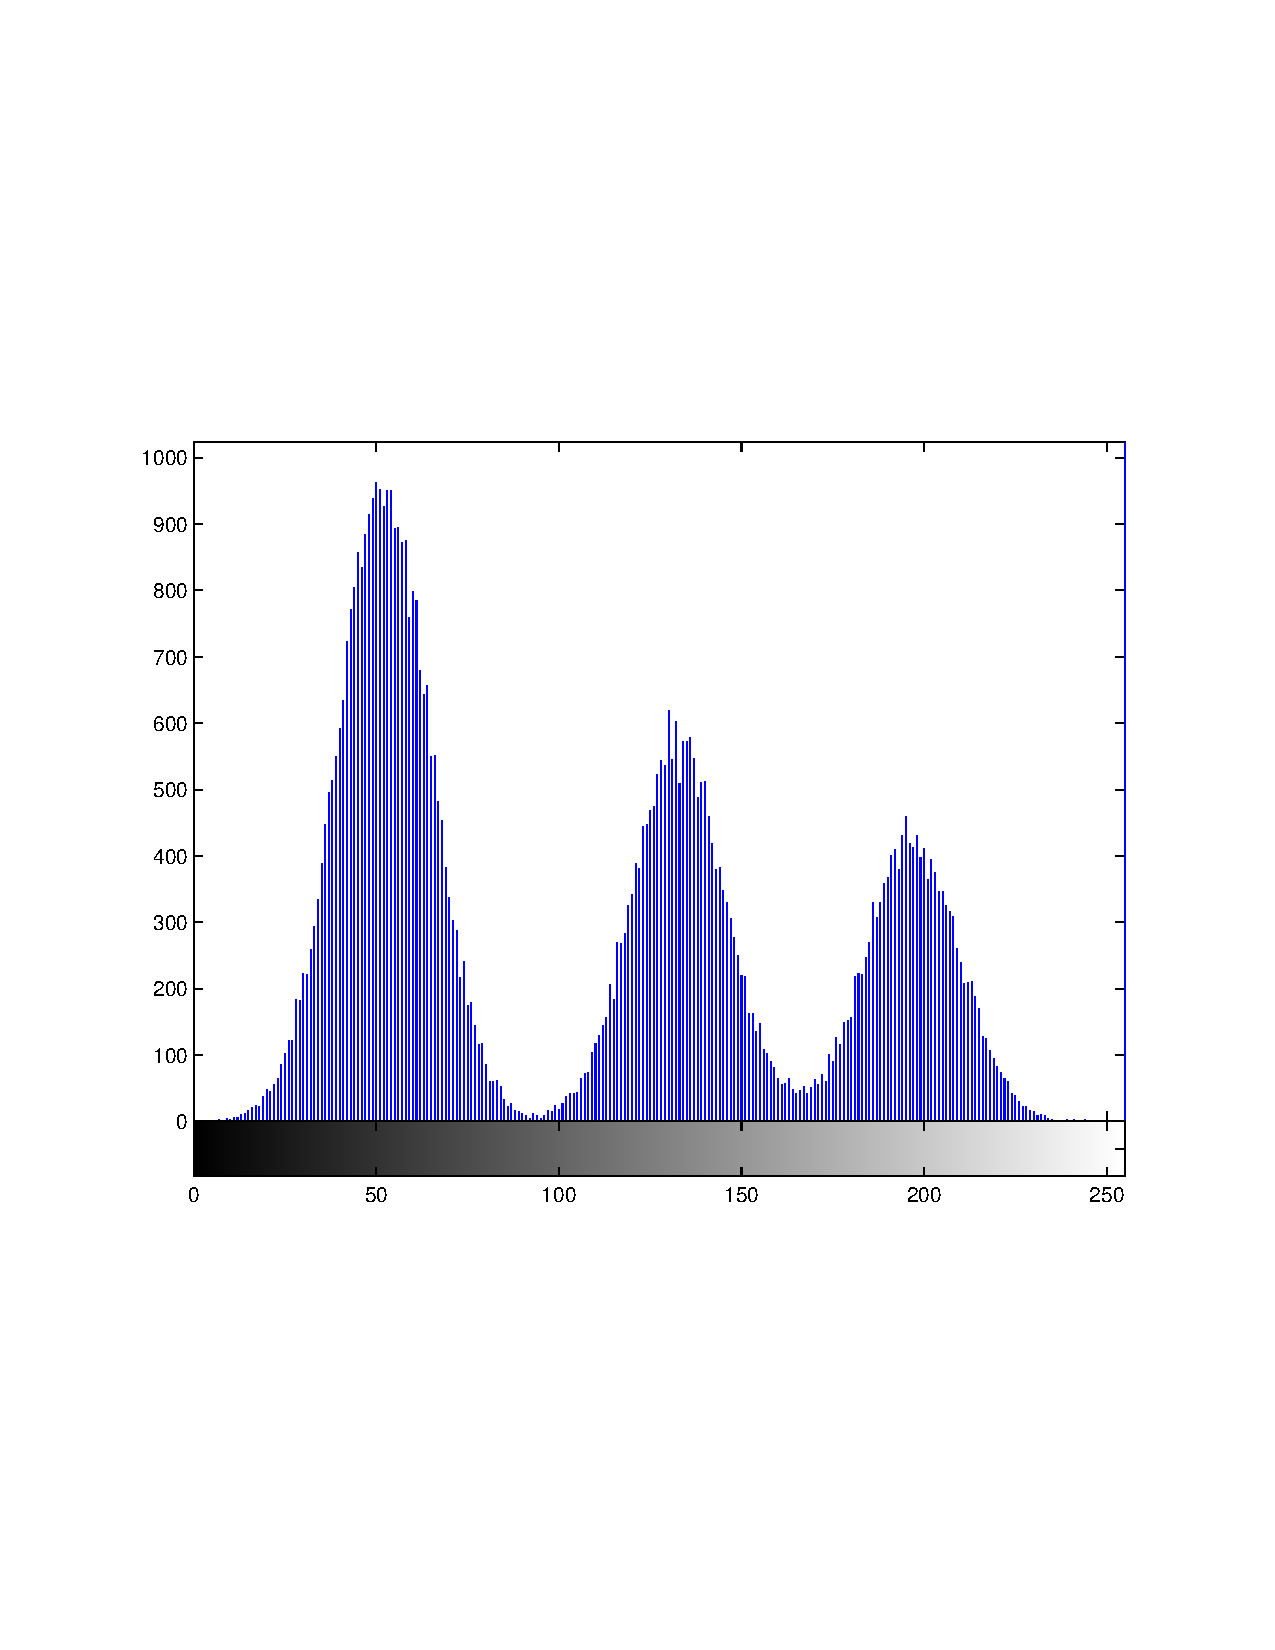
\includegraphics[width=0.4\textwidth]{q2-boxhist.pdf}}
%\subfloat[Histogram after filtering]{\label{fig2:boxfinalhist}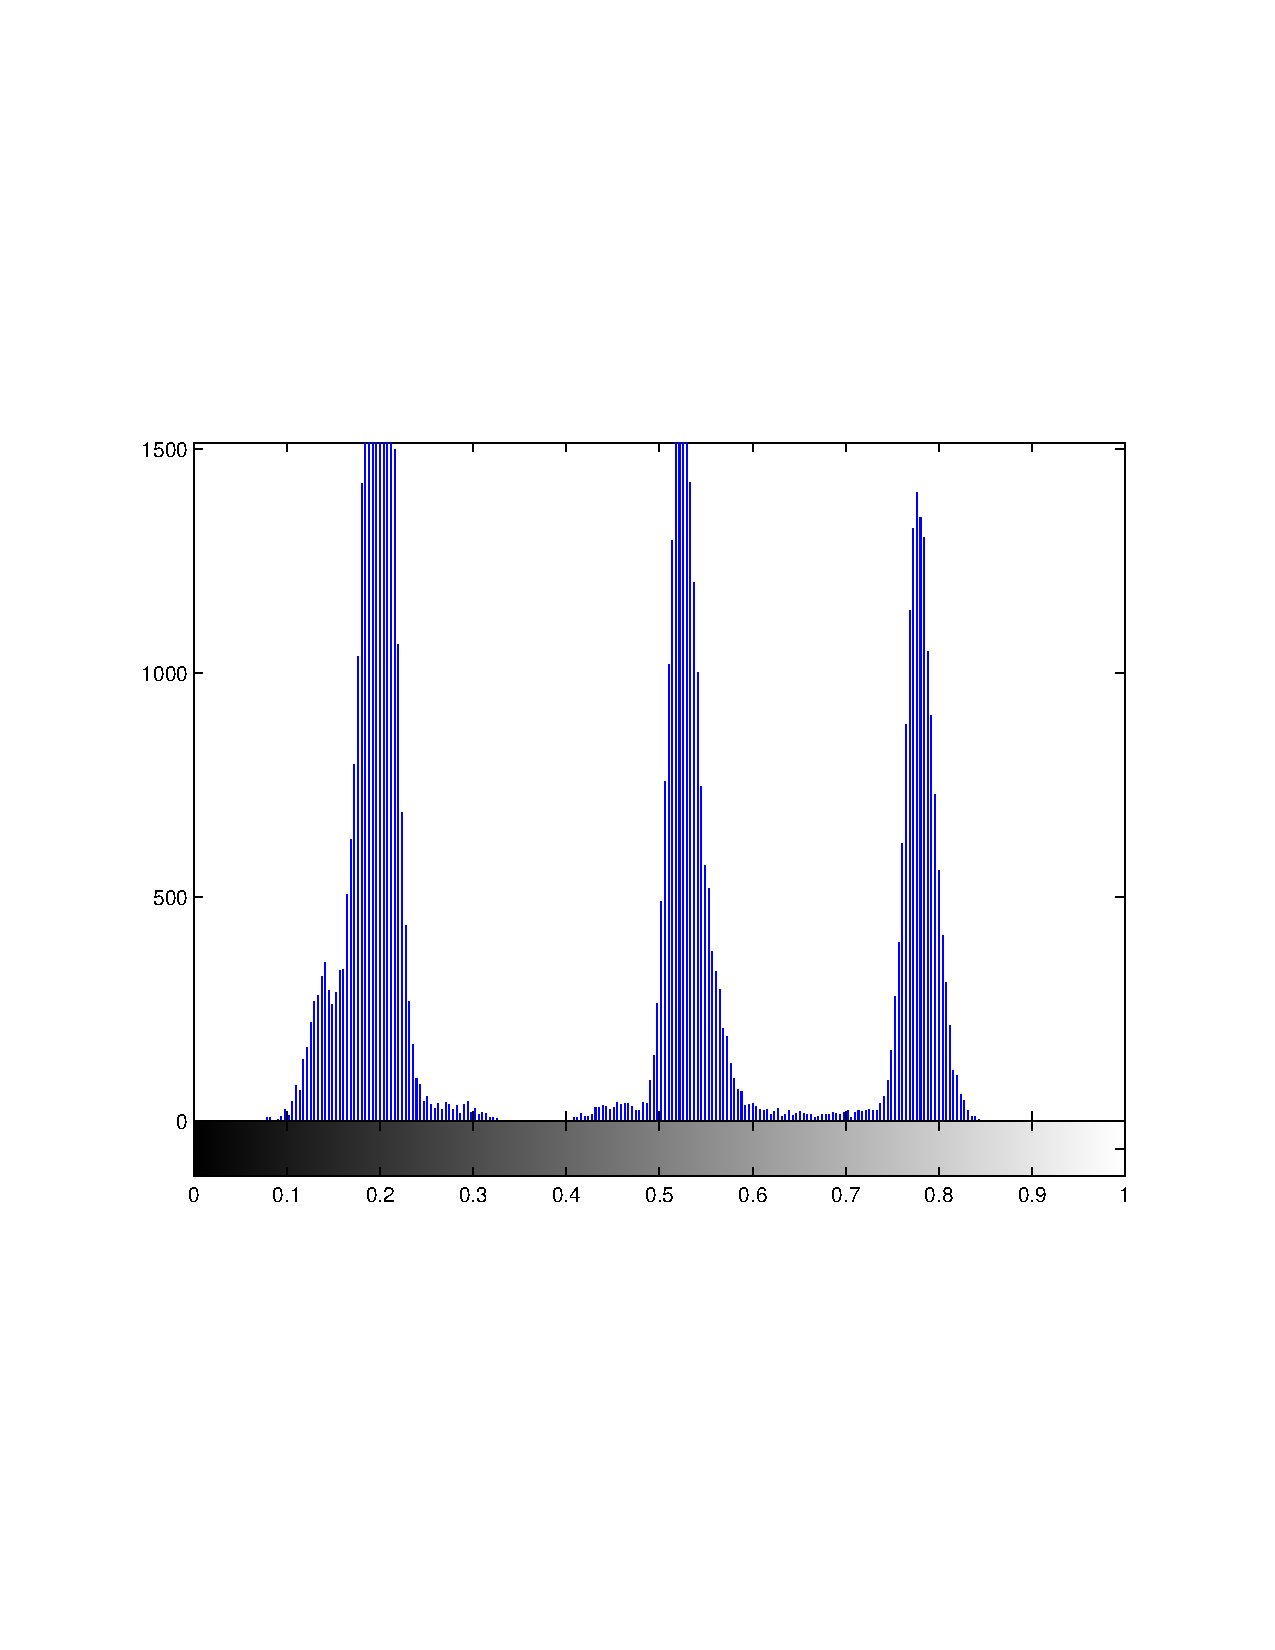
\includegraphics[width=0.4\textwidth]{q2-boxhist-after.pdf}}
\caption{Applying the wiener2 function to boxes.tif}
\label{q2:boxes}
\end{figure}

\section*{Question 3.3 - Long exposure blurring}
\subsection*{(a)}
The sky.tif image shows star trails: the blurs resulting from a long exposure of the night sky. The source of the degradation in this image in particular is the rotation of the camera/telescope relative to the galaxy it is photographing. As the camera is pointing towards the centre of the rotation then the blue turns out to be circular.

The process is almost linear in that the star pixels have all rotated in the same way (by the same angle and the same distance). The degradation process is almost shift invariant because if an input (a star for example) moves, then the output (the blurred star) will also be moved. The reason the effect on the entire image is not linear and shift invariant is that it is only the stars which are affected: the other parts of the image have not moved and are therefore not linearly effected.

There is also some noise present in the image - given that it is a long exposure photograph I would expect some element of this to be present.

\subsection*{(b)}
Estimating the location of the pole by visual inspection gave the coordinates (440,335).

The exposure time can be estimated using the fact that stars rotate 2.5\textdegree per 10 minutes and then measuring the pixels of one of the stars (source: \url{http://www.jmg-galleries.com/blog/2011/11/22/pro-tip-calculating-unknown-star-trail-exposure-times/}).

For this image I used a Matlab plugin (image measurement utility - \url{http://www.mathworks.com/matlabcentral/fileexchange/25964}) to open a window and measured the angle from the estimated centre to both ends of one of the trails, as can be seen in figure \ref{q3:measure}. I measured this at 8.84\textdegree, and the calculation $ \frac {angle} {2.5} * 10 \text{ minutes}$ gave the estimate 35 minutes and 21.6 seconds.
	
	\begin{figure}[h!]
		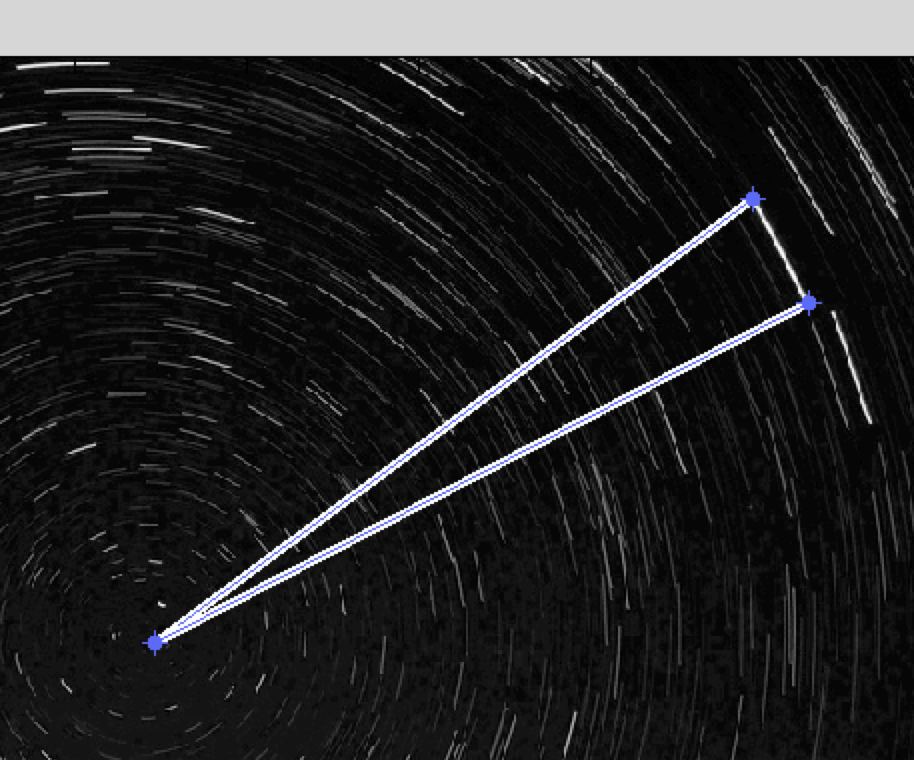
\includegraphics[width=0.3\textwidth]{q3ss.png}
		\caption{Measuring the angle}
		\label{q3:measure}
	\end{figure}
	
	
\subsection*{(c)}
If the image is processed as specified with Tikhonov regularised least squares error, it will be problematic to implement inverse Fourier filtering because of the potential of division by zero, caused by the many black pixels in the sky. As the values tend towards 0, the restored image values (in the Fourier domain) will tend toward infinity.

\subsection*{(d)}
It should be possible to use Wiener filtering in the Fourier domain to recover the sky, as the predominant degradation of the image is known (in this case we have measured the rotation to help determine the inverse filter for the blur). One could estimate the noise parameters by examining a plain area of the sky (containing no stars) to determine a noise mask. By subtracting the image taken in a much shorter exposure (i.e. instantaneous) and subtracting this from the long exposure, only the difference caused by the rotation should be remaining (assuming a similar exposure of the two images). This gives an image without the foreground elements and allowing the Wiener filtering a better chance to recover the instantaneous sky. Assuming this works, the original image could then be created by adding the Wiener filtered result to the short exposure image to give both the foreground and the recovered instantaneous sky.

This assumes that the rotation of the camera is precisely aligned such that the degradation can be accurately modelled. In addition, we must assume that the stars did not change appearance during the exposure, but only changed in their position in the sky. The atmosphere must also remain fairly constant - the optimal case is that the photograph is taken away from artificial light sources and on a clear night.

\section*{Question 3.4 - Restoration}
The first part of the problem is to build an experimental model of the image degradation. This model has the form of a function $H(u,v)$ which represents a filter on the original image.

Inspecting the wood.tif file reveals quite a lot of blurring.  In the horizontal direction, the pixels are blurred more than in the vertical direction. The blur is not diagonal (the camera does not appear to have moved diagonally relative to the image). If looks a little like the lens was not focussed correctly or some low pass blur filtering has been applied, such as the Gaussian low pass. 

I built a model of the blurring as the product of a horizontal motion blur of 5 pixels and a vertical motion blur of 6 pixels. The result of applying this model with regularised deconvolution is shown in figure \ref{q4ish}. This image retains a lot of noise but appears a little sharper. Not all of the motion blur has been removed and the noise level was measured (by inspecting an area of pixels on one brick) with variance 0.0013. This is a long way from the target of 1.

In order to take into account the smoothness of the x-direction blur, I then tried to change the regularisation parameter to use a modified Laplacian operator, by decreasing the horizontal gradient of the laplace matrix - the result is in figure \ref{q4ish2}. This made the vertical lines slightly better defined.

I was not sure how to proceed after this. The noise variance of the latter image increased to 0.0028 but this was still a long way from the target of 1. I estimated the $\gamma$ value incrementally using the algorithm from Gonzalez and Woods (page 360) but this did not seem to give the correct results, and took a long time to compute (and after 500 iterations had not reached a good value). The initial value of 0.001 seemed to be fairly good though.

I tried using the image processing toolbox method deconvblind, which takes an image and an initial model of the point spread function, and applied it using my combined horizontal and vertical blur. It did not add noise as previously, however the blur removal was similar to that of the regularised result. The result is shown in figure \ref{q4ish4}. 

At this point I ran out of time for this question and could not think how to improve my results.

\begin{figure}[h]
\subfloat[Original image]{\label{fig4:wood}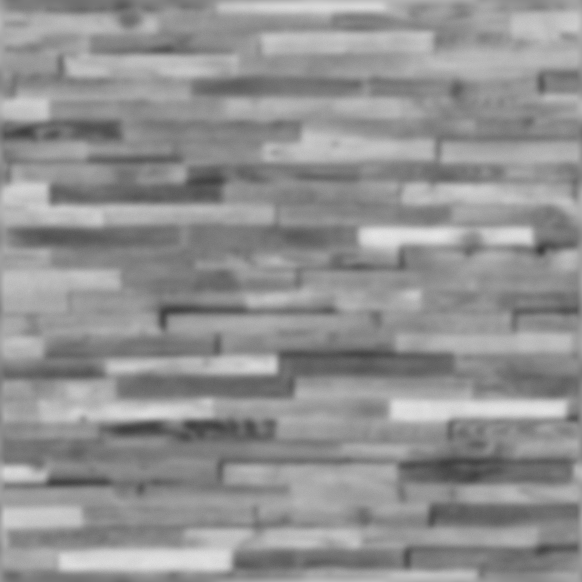
\includegraphics[width=0.3\textwidth]{q4-wood.png}}\qquad
\subfloat[Restored image with regularised deconvolution, Tikhonov]{\label{q4ish}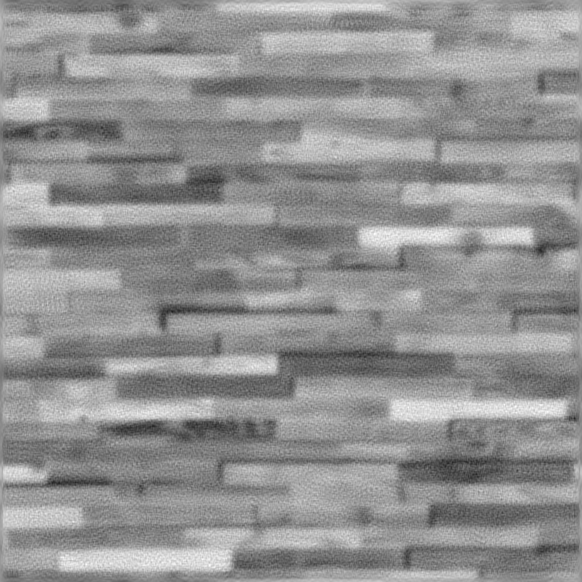
\includegraphics[width=0.3\textwidth]{q4-defilteredmotion.png}}\qquad
\subfloat[Restored image with regularised deconvolution, changed laplace]{\label{q4ish2}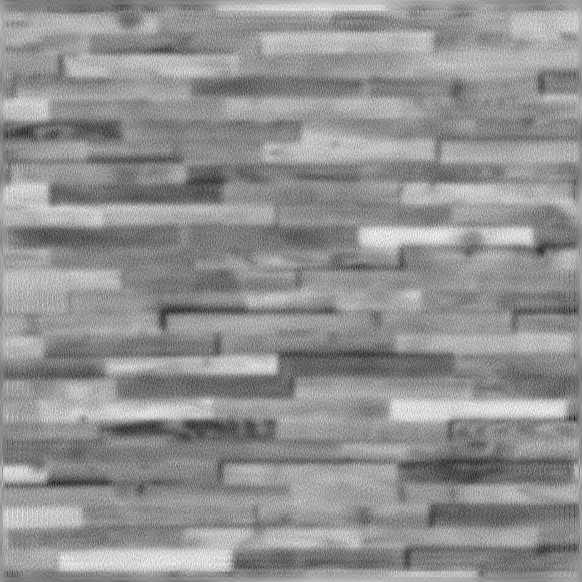
\includegraphics[width=0.3\textwidth]{q4-defilteredmotion-lapmod.png}}\\
\subfloat[Restored image with regularised deconvolution, changed laplace]{\label{q4ish4}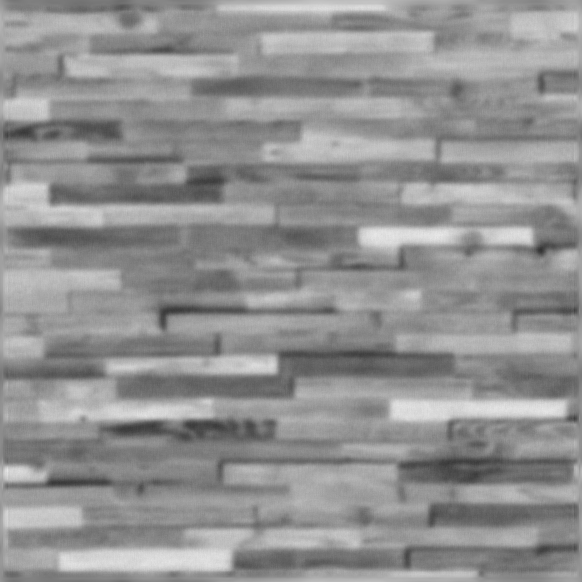
\includegraphics[width=0.3\textwidth]{q4-blind.png}}
\caption{Applying the deconvolution with motion blur in 2 directions to wood.tif}
\label{q4}
\end{figure}

\break
\appendix
\section{Figures for question 3.1}

\begin{figure}
\subfloat[Gaussian samples ($\mu = 0$, $\sigma = 0.5$)]{\label{fig1:gauss}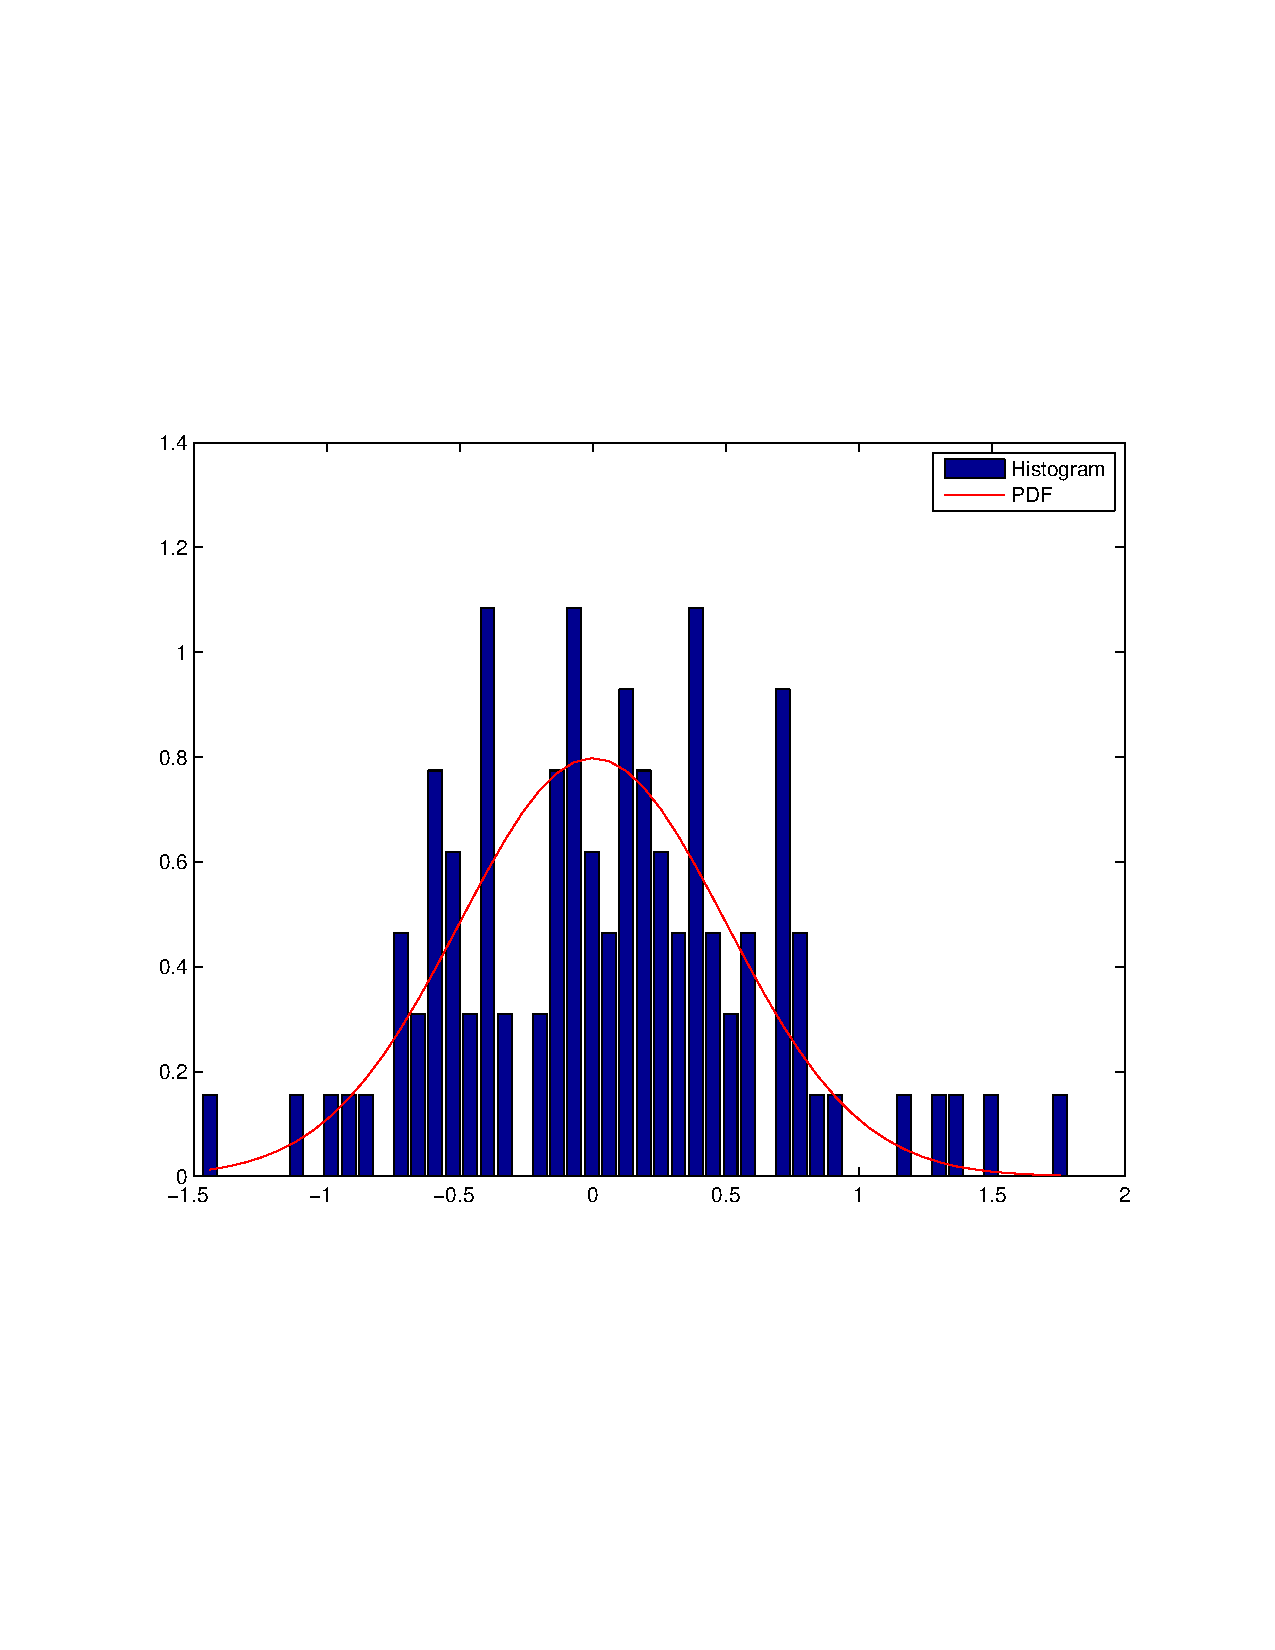
\includegraphics[width=0.5\textwidth]{q1-gaussian.pdf}}
\subfloat[Gamma samples ($a = 1$, $b = 1$)]{\label{fig1:gamma}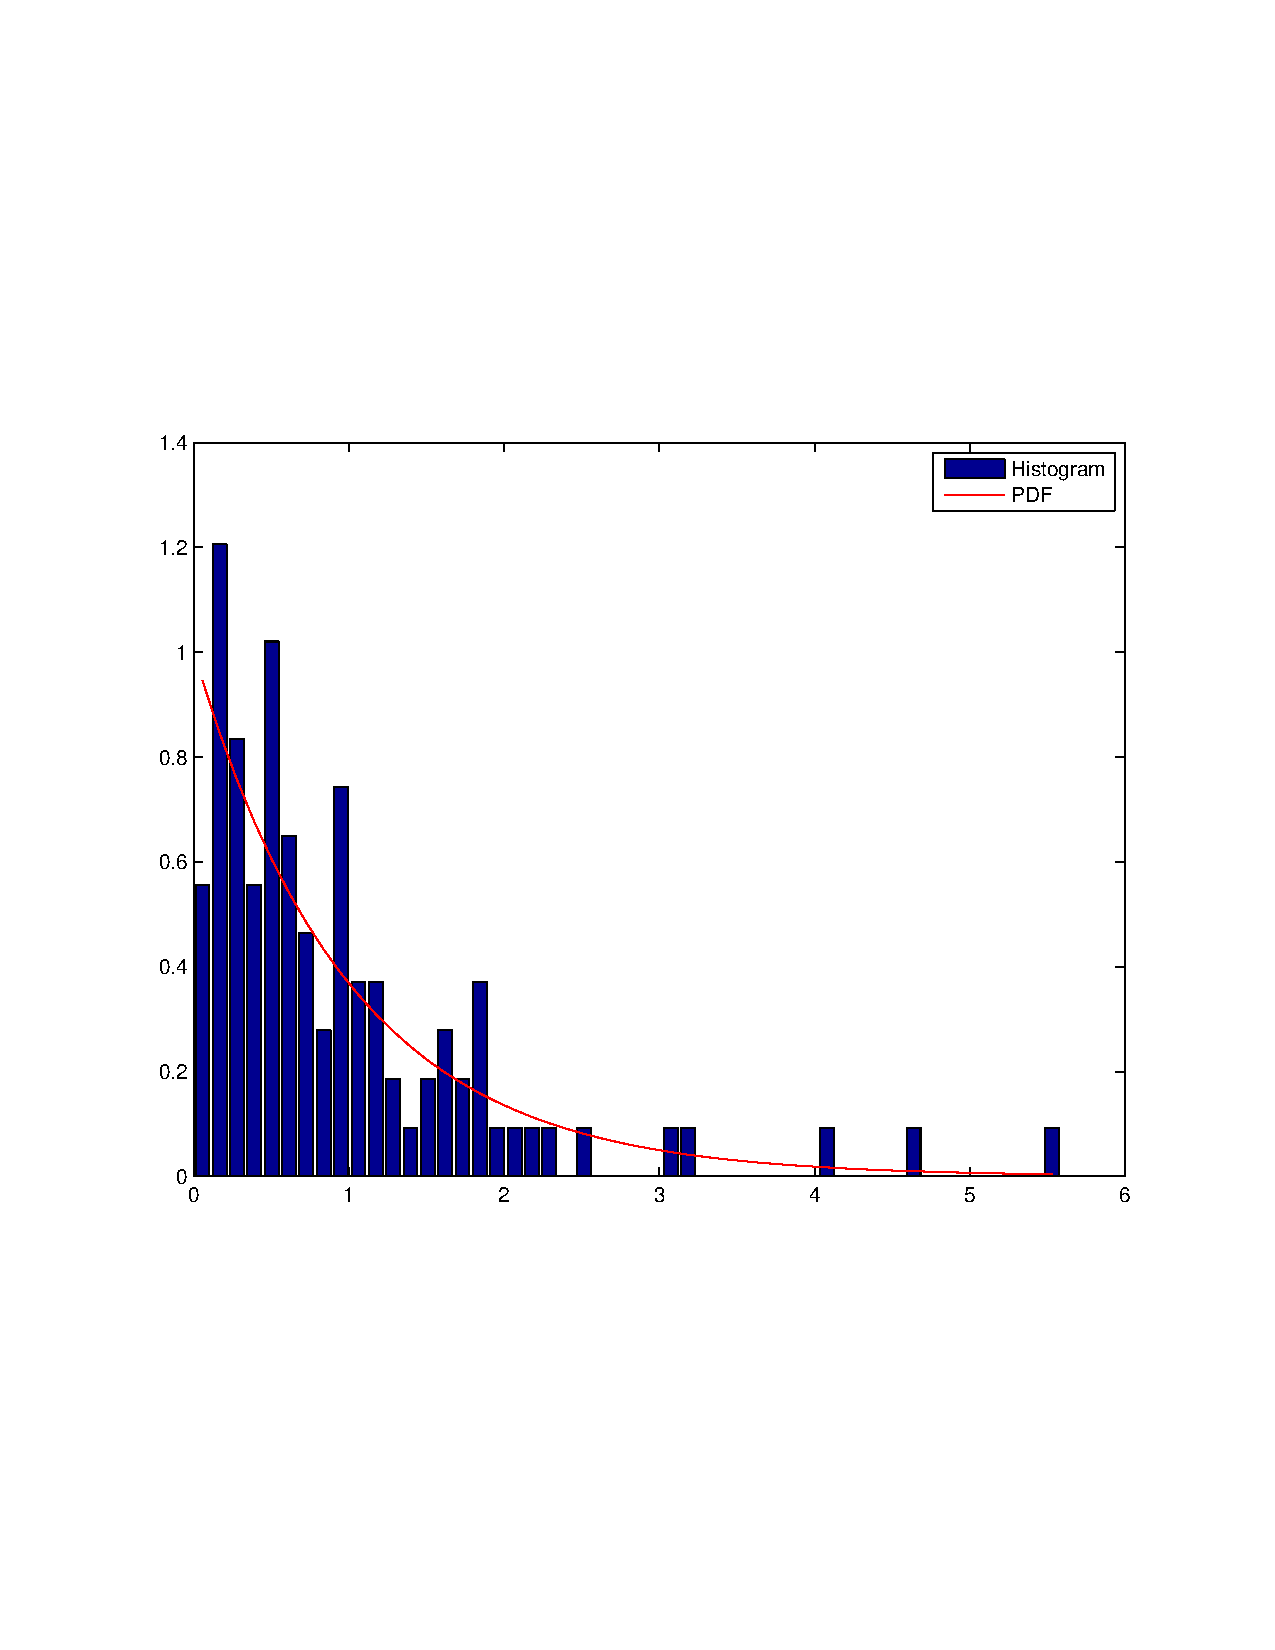
\includegraphics[width=0.5\textwidth]{q1-gamma.pdf}}\\
\subfloat[Uniform samples ($a = 0$, $b = 2$)]{\label{fig1:uniform}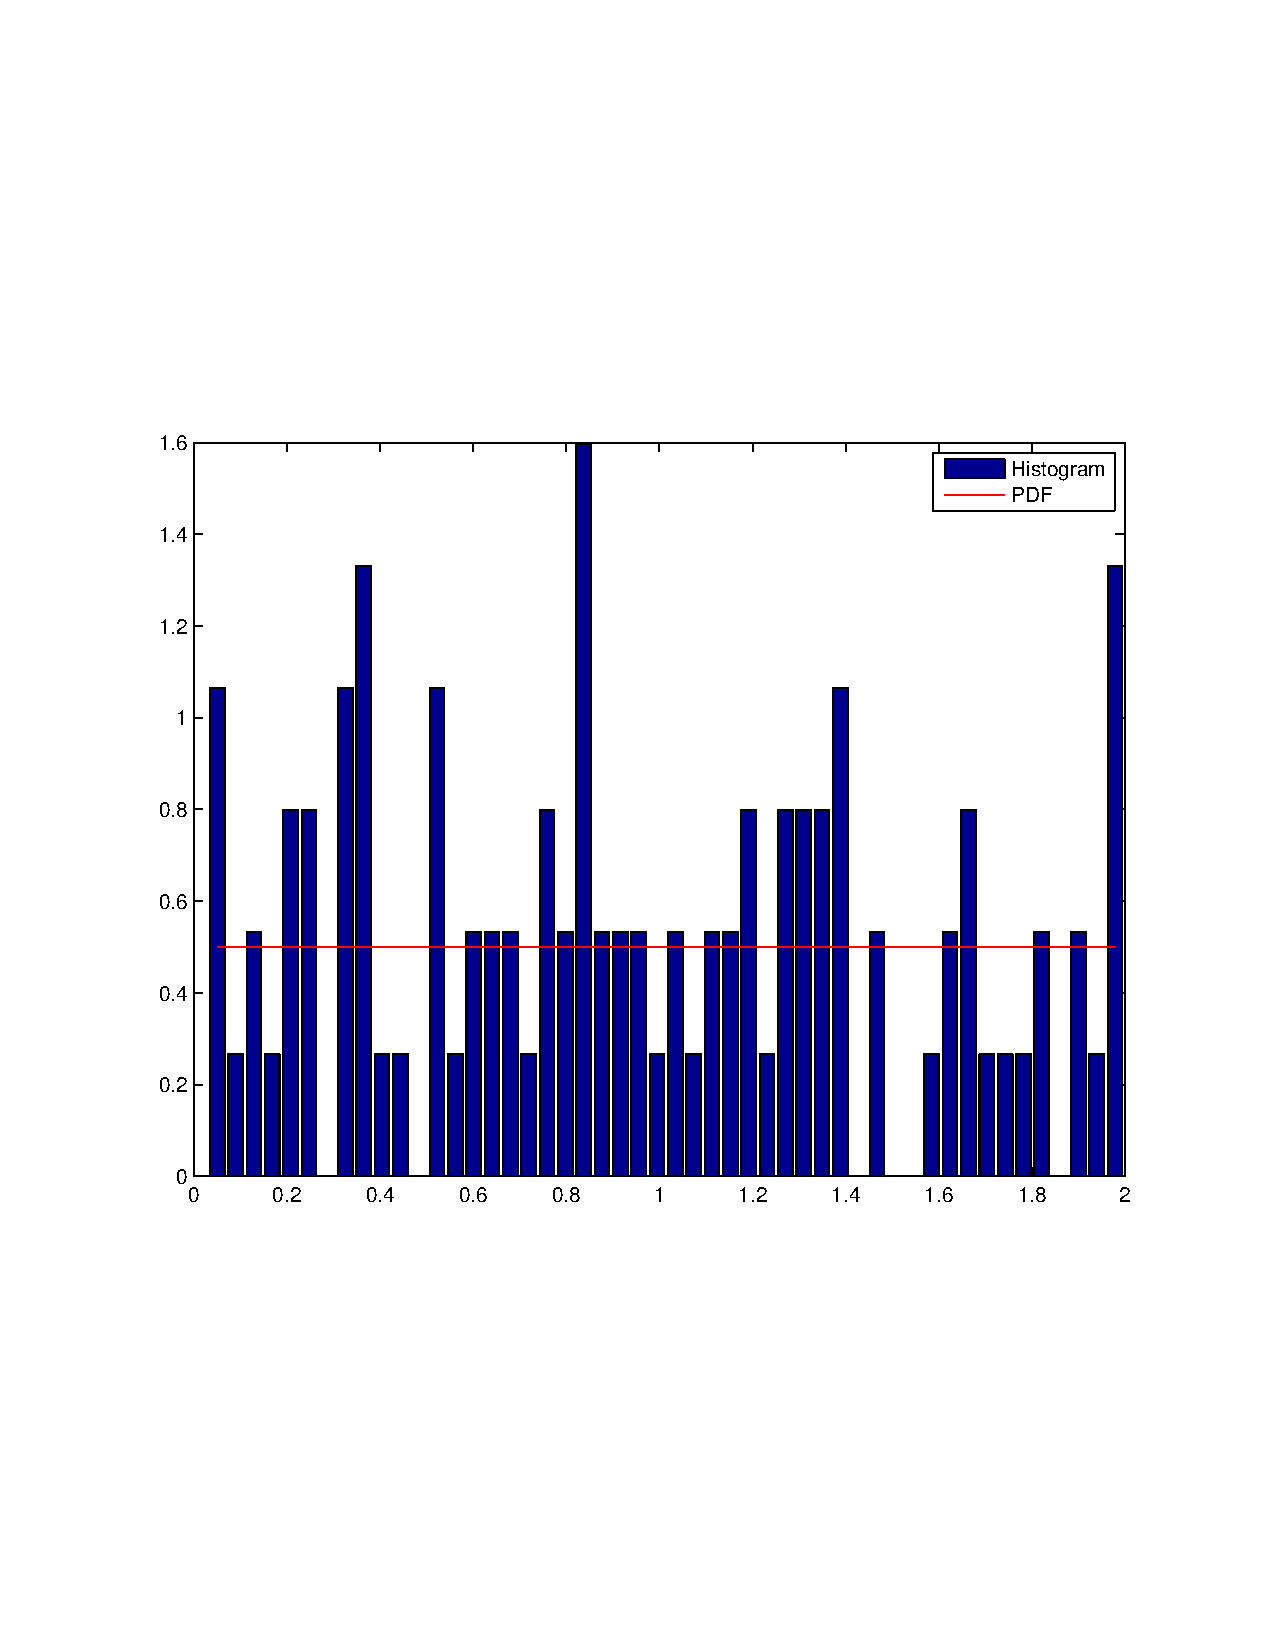
\includegraphics[width=0.5\textwidth]{q1-uniform.pdf}}
\subfloat[Salt \& Pepper samples ($P_0 = 1/3$, $P_2 = 2/3$)]{\label{fig1:sandp}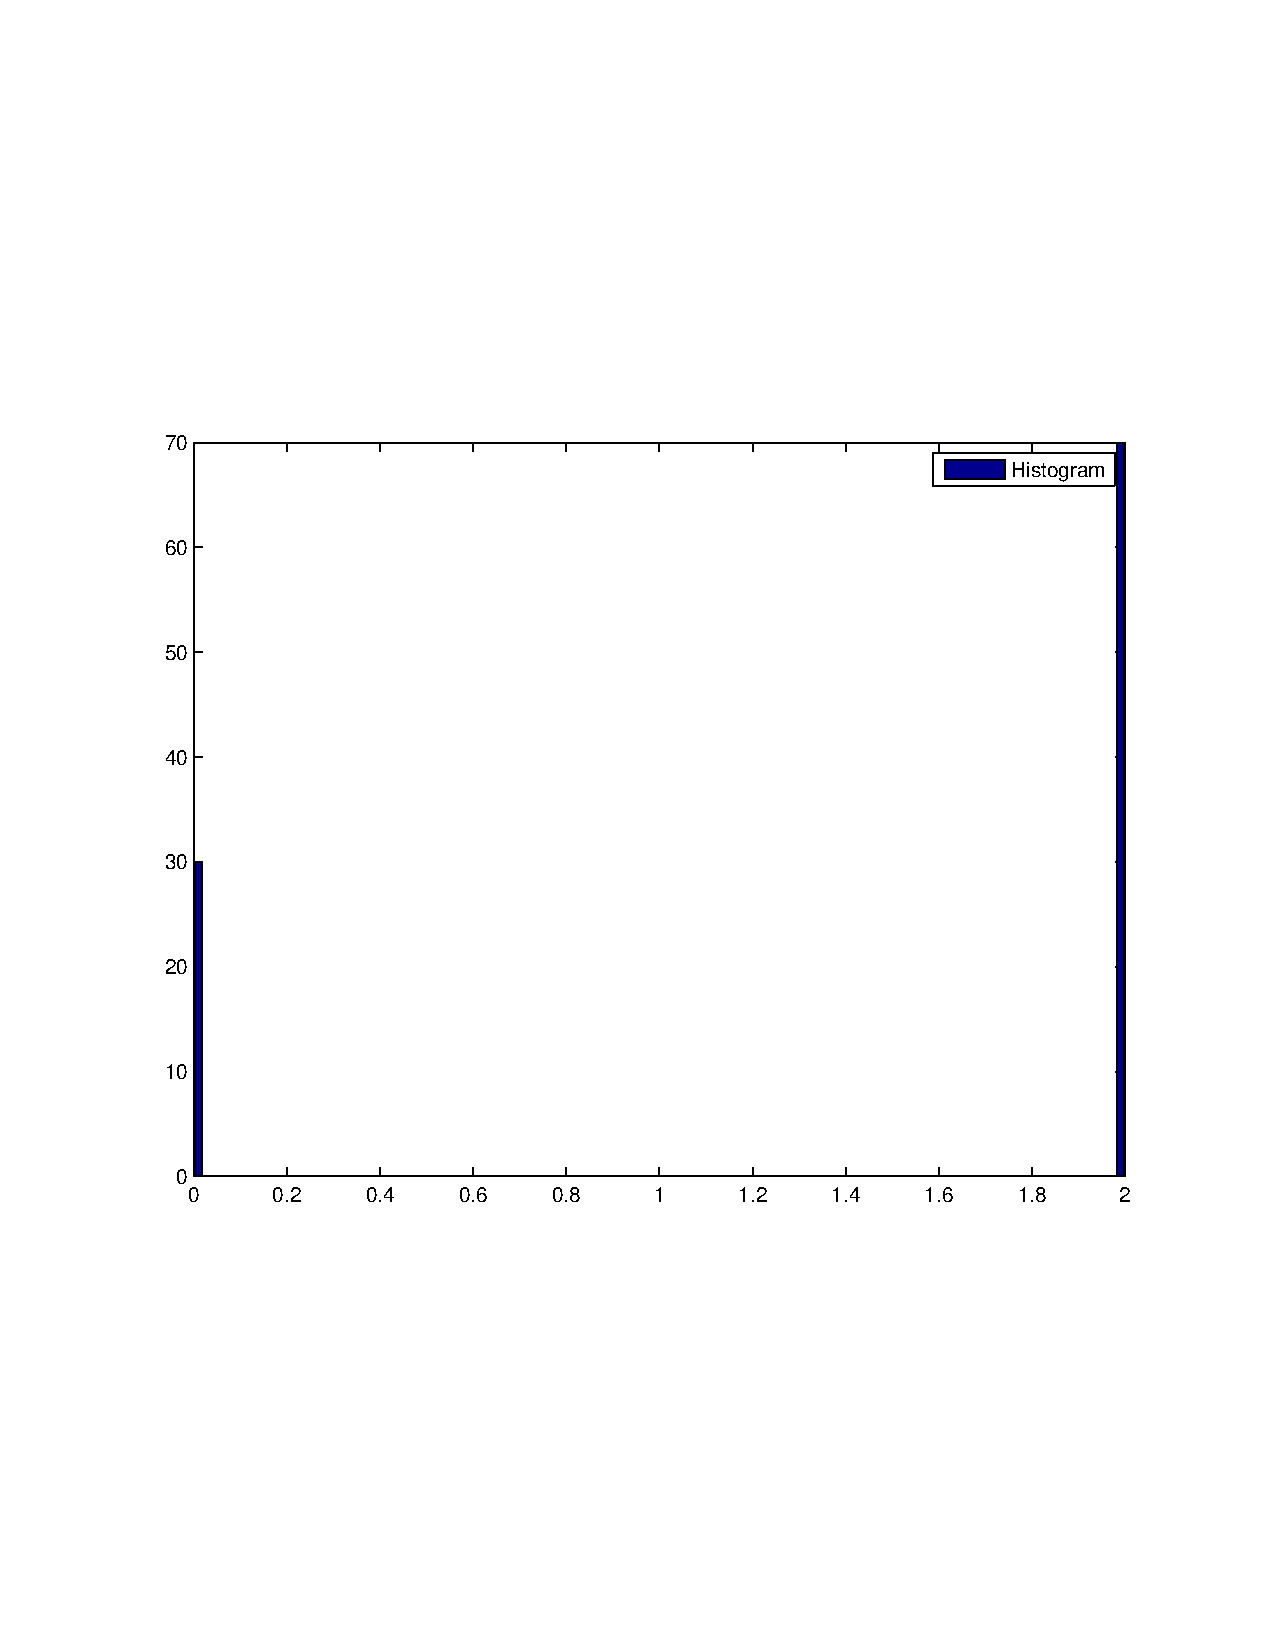
\includegraphics[width=0.5\textwidth]{q1-sandp.pdf}}
\caption{Histograms for noise samples in question 3.1}
\label{fig:q1}
\end{figure}

 \end{document}
